\chapter{总体概述}


\section{软件概述}
\subsection{项目介绍}


本音乐播放系统是一个全新的项目,旨在为用户提供一个可以随时随地通过互联网播放,购买,评价音乐,创建喜欢的歌单,获得专属音乐推荐以及和朋友分享音乐的应用程序。\\


本产品是独立的并且完全自我包含的。\\
本项目的主要组件包括:
\begin{itemize}
\item \textbf{用户终端:}通过网络向服务器发送请求,从服务器接受数据,并为用户呈现出来。用户终端的环境是网页浏览器。
\item \textbf{服务器:}接受和处理客户端发来的请求,根据用户的请求从数据库提取信息,并将处理过的信息发送给客户端,或者根据客户端发送的请求更新数据库中的信息。服务器的主要接口包括:
\begin{itemize}
\item \textbf{用户信息接口}:用于用户信息的传递,验证和修改。
\item \textbf{交易接口}:主要用于结算功能,本接口需要稳定和安全。
\item \textbf{下载接口}:用户应该通过该接口获得下载文件。
\item \textbf{在线播放接口}:用户可以通过该接口获取在线播放的服务。
\end{itemize}
\item \textbf{数据库:}一个SQL Server数据库,仅可以由服务器访问,存储本系统的各种信息。主要包括:
\begin{itemize}
\item \textbf{用户信息}:包括用户的ID,用户名,密码,权限等信息。
\item \textbf{歌单信息}:包括用户自建歌单,用户分享的歌单,用户购物车等等信息。
\item \textbf{音乐信息}:音乐的相关信息,包括艺人,所属专辑等等。
\item \textbf{音乐文件}:存储音乐数据文件。
\item \textbf{评价信息}:存储用户对音乐的评价,可以用于推荐。
\end{itemize}
\end{itemize}

\section{软件功能}
\subsection{文字说明}
本项目的主要功能包括:
\begin{itemize}
\item \textbf{一、音乐播放}
\begin{itemize}
	\item \textbf{在线播放}支持在线音乐播放
\end{itemize}
\item  \textbf{二、浏览和搜索部分:}
\begin{itemize}
	\item \textbf{浏览目录:}用户可以根据风格,专辑或者艺术家来分类浏览音乐。
	\item \textbf{音乐搜索:}用户可以根据音乐的名称,风格,艺术家,专辑等信息搜索对应的音乐作品。
	\item \textbf{推荐歌曲:}用户可以获得专属的音乐推荐。
	\item \textbf{排行榜:}服务器根据播放信息和评分信息生成音乐排行榜,用户可以查看该榜单。
\end{itemize}
\item \textbf{三、账户管理:}
\begin{itemize}
	\item \textbf{账户注册}
	\item \textbf{账户登录:}用户有不同的权限,普通用户登录将进入用户主界面,管理员登录将进入管理员页面。
	\item \textbf{账户注销}
	\item \textbf{账户信息编辑:}信用卡信息。
\end{itemize}
\item \textbf{四、音乐购买和下载:}
\begin{itemize}
	\item \textbf{音乐加入购物车}
	\item \textbf{查看和编辑购物车}
	\item \textbf{账单结算}
	\item \textbf{音乐下载:}用户可以下载已购买的音乐。
\end{itemize}
\item \textbf{五、歌单管理:}
\begin{itemize}
	\item \textbf{歌单创建:}用户可以创建多个属于自己的歌单。每个用户都固定拥有一个已购买歌单。
	\item \textbf{向歌单添加音乐:}用户可以将音乐添加到指定的歌单中。
	\item \textbf{从歌单删除音乐:}用户可以删除歌单中的音乐。
	\item \textbf{歌单删除:}用户可以删除一个歌单。(已购买歌单不能删除)
\end{itemize}
\item \textbf{六、音乐分享:}
\begin{itemize}
	\item \textbf{歌曲分享}用户可以将歌曲、歌单或专辑分享给自己的朋友。
	\item \textbf{查看分享信息}用户可以在分享查看页面查看其他用户分享给自己的音乐,歌单和专辑。
\end{itemize}
\item \textbf{七、音乐评价:}
\begin{itemize}
	\item \textbf{音乐评价:}每一个用户都可以对任何一首音乐进行评分。
	\item \textbf{查看音乐评价:}用户可以查看任意一首歌的评价信息
\end{itemize}
\item \textbf{八、管理员功能:}
\begin{itemize}
	\item \textbf{}给与其他用户管理员权限
	\item \textbf{}删除音乐,类别,艺术家和专辑
	\item \textbf{}添加类别,艺术家和专辑。
	\item \textbf{}上传音乐。
\end{itemize}
\end{itemize}

\subsection{用户用例图}
使用以下用例图显示用户各个功能:
\begin{figure}[ht]
	\centering
	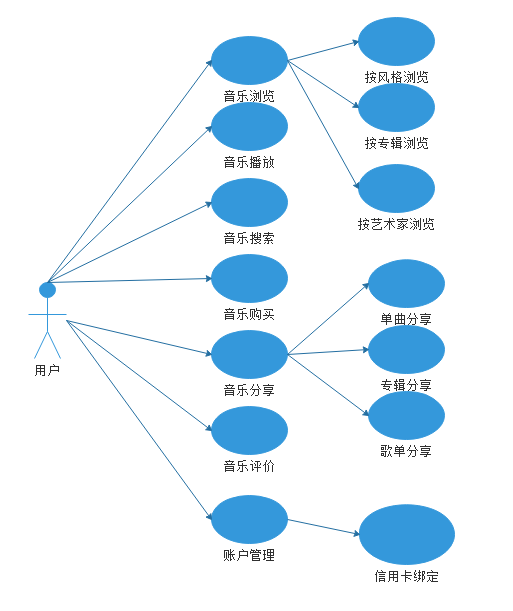
\includegraphics[width=10cm]{User.png}
	\caption{用户功能图} \label{fig:figure1}
	\end{figure}



		
\subsection{页面流图}
为了说明各个页面之间的关系,绘制了如下页面流图:
\begin{figure}[ht]
	\centering
	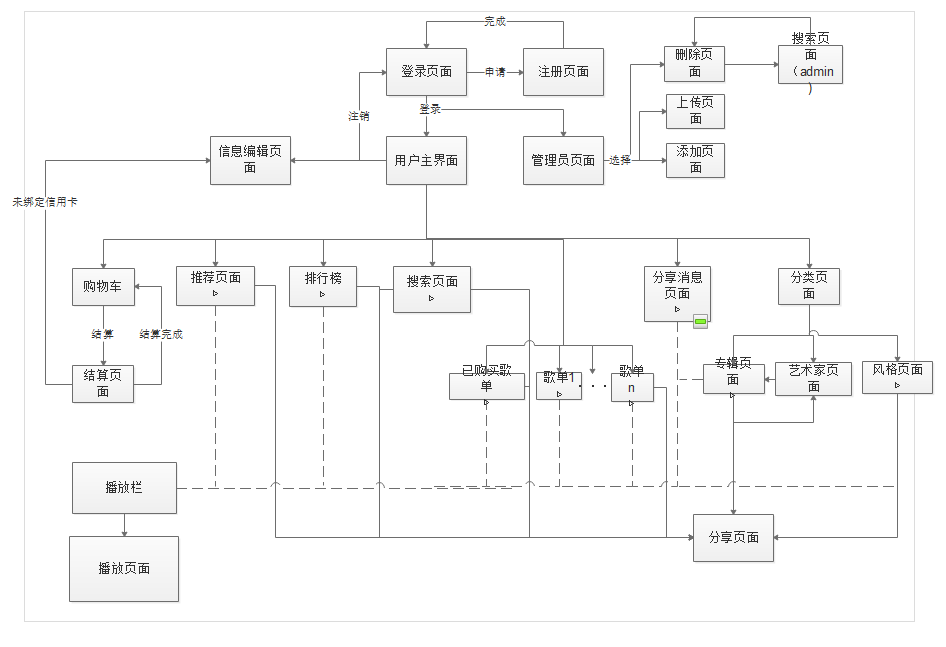
\includegraphics[width=10cm]{Pageflow.png}
	\caption{页面流图} \label{fig:figure3}
	\end{figure}


	
\subsection{页面说明}
其中,播放栏是悬浮在网页下方的一个小型页面,是最小化的播放页面,如果某个页面有虚线与播放栏相连,代表该页面和播放栏共存,从播放栏可以跳转到放大的播放页面。


各个页面能完成的功能如下:
\begin{itemize}
	\item \textbf{登录页面:}登录和注册账户
	\item \textbf{管理员页面}:选择进入删除、上传,还是添加页面
	\item \textbf{删除页面:}可以向数据库删除音乐,风格,艺术家等
	\item \textbf{添加页面:}可以向数据库添加音乐,风格,艺术家等
	\item \textbf{上传页面:}可以上传音乐
	\item \textbf{用户主界面:}可以选择进入,购物车,推荐,排行榜等界面。
	\item \textbf{信息编辑页面:}可以编辑用户的用户名,密码,信用卡号等基本信息。
	\item \textbf{购物车页面:}可以查看用户的购物车。
	\item \textbf{结算页面:}结算账单,若未绑定信用卡信息则跳转到信息编辑页面。
	\item \textbf{分类页面:}按专辑,艺术家或者风格浏览音乐。
	\item \textbf{艺术家页面:}浏览艺术家的所有专辑。
	\item \textbf{播放页面:}可以在线播放/暂停,可以进行评价。
	\item \textbf{分享页面:}输入用户要分享的用户,确认即可分享。
\end{itemize}
以下页面和播放栏共存,并且都有下载,将音乐加入购物车和分享的功能。\\
如果点击分享功能,就选定了分享的内容,并跳转到分享页面输入要分享的用户即可。\\
除此以外各个页面还拥有以下功能:
\begin{itemize}
\item \textbf{推荐页面:}查看系统对用户推荐的音乐。
\item \textbf{排行榜:}查看音乐排行榜。
\item \textbf{搜索页面:}根据用户输入的信息搜索音乐。
\item \textbf{歌单页面:}查看用户的各个歌单。
\item \textbf{分享消息页面:}可以查看其他用户对当前用户分享的音乐,歌单和专辑。
\item \textbf{专辑页面:}查看某个专辑的所有音乐。
\item \textbf{风格页面:}查看某种风格的音乐。
\end{itemize}

\section{用户特征}

\begin{itemize}
	\item \textbf{用户经验:}	本系统面向的用户是拥有基本电脑操作能力的用户。用户需要拥有使用鼠标和键盘的经验。
	\item \textbf{用户能力:} 用户需要有互联网连接。
	\item \textbf{用户角色:}	在本系统中,用户扮演的角色主要是消费者。用户可以在线播放音乐,购买、下载和上传音乐,评价音乐,管理和分享自己的歌单等等。但是用户不能修改服务器上歌曲,专辑,艺人等的信息。
\end{itemize}
\section{假设和依赖关系}


外部依赖:

\begin{itemize}
	\item \textbf{}本项目是一个独立的完全包含的项目,不重用其他项目模块。
	\item \textbf{}本项目的将主要使用C\#和ASP.NET编写。
	\item \textbf{}本项目的开发环境将是Visual Studio 2017。
	\item \textbf{}本项目将在Windows10平台下测试。
	\item \textbf{}本项目中的数据文件格式使用xml格式。
\end{itemize}
假设:

\begin{itemize}
	\item \textbf{用户}
	\begin{itemize}
		\item \textbf{}用户界面使用ASP.NET生成的Web页面。用户需要安装Microsoft .NET Framework。
		\item \textbf{}用户使用本系统时应该拥有Internet连接。
	\end{itemize}
	\item \textbf{服务器}
	\begin{itemize}
		\item \textbf{}系统部署在IIS服务器上。
	\end{itemize}
	\item \textbf{数据库}
	\begin{itemize}
		\item \textbf{}使用Microsoft SQL数据库服务器。
	\end{itemize}
\end{itemize}	